\chapter{Installation}

\section{Prerequisites}
Since \oxdoc~was written in Java, you should have Java installed on your computer.  
The fact that \oxdoc~is a Java program means that it can in principle be used on 
any operating system, including Windows and Linux. In this section, the installation
process for Windows operating systems will be described. 
For Linux and other operating systems, we will describe the manual installation 
process which is slightly more complicated.

The Java Runtime Environment (JRE) can be downloaded from {\tt www.java.com/getjava}.
Most Linux distributions either have Java pre-installed, or it can be installed from
the installation repositories.

In order to use \LaTeX~generated formulas, a copy of \LaTeX~is required as well.
A free Windows distribution called MiKTeX can be downloaded from {\tt http://www.miktex.org/}.
Alternatively, \oxdoc~can generate mathematical formulas using the JavaScript package
MathML. Generating formulas with MathML does not require any third-party software. 

\oxdoc~uses a program called \dvipng~to generate PNG (Portable Network
Graphics) files from \LaTeX~code.  The full installation of MiKTeX comes with a version
of this programs, but other distributions may not have it readily available.  If you
use a non-full installation of MiKTeX, make sure to select \dvipng~during the
installation. Most Linux distributions have \dvipng~in their installation repositories. For
example, installing \dvipng~on Ubuntu would be done by issuing the following command in a terminal:
\begin{quote}
\tt sudo apt-get install dvipng
\end{quote}

\section{Installation}
\subsection{Installation on Windows 2000/XP}
Follow the following steps to install \oxdoc:
\begin{enumerate}
\item Download the latest binary zip file ({\tt oxdoc-xxxx-bin.zip}) from
the SourceForge website \\({\tt http://oxdoc.sourceforge.net}). 
\item Unzip this file in a convenient directory
(for example in {\tt C:\bs Program Files\bs oxdoc}). 
\item Run the set up program. This program can be found in the subdirectory {\tt oxdoc\bs bin}
in the directory in which you installed \oxdoc. Double-click on {\tt setup.bat} to start it.
You will see the following setup screen:
\begin{center}
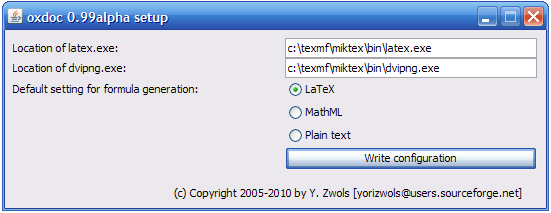
\includegraphics[scale=0.5]{setup_win.png}
\end{center}
\item Make sure to specify the location of the {\tt latex.exe} and {\tt dvipng.exe} files
of your MiKTeX installation (or any other \LaTeX~distribution). 
\item Click `Write configuration' to save the options to the main \oxdoc~configuration file
(i.e. a file named \oxdocxml~that is located in the `{\tt bin}' subdirectory of the \oxdoc~intallation.)
\item (Optional) You may also want to add the \oxdoc~directory to your search path, so that \oxdoc~can
be run from any working directory. To do so, right-click on the `My Computer' icon
on your desktop, and choose `Properties'. Under the tab `Advanced', click on the
button `Environment Variables'. Edit the variable `Path' which can be found under System 
variables by adding a semi-colon followed by the path to the {\tt bin} subdirectory 
of your \oxdoc~installation. For example, your path may now look like:
\begin{quote}\tt
	\%systemroot\%\bs system32;\%systemroot\%;C:\bs program files\bs oxdoc\bs bin
\end{quote}
Click OK a couple of times to commit the changes. Notice that the changes will not
affect only newly opened command line windows, so that all already opened command line
windows will not notice the changes.
\end{enumerate}

You are now ready to use \oxdoc. In the subdirectory {\tt oxdoc\bs bin}
you can find the \oxdoc~graphical user interface that helps you get started
with running \oxdoc. 
To test whether \oxdoc~works, run the batch file {\tt oxdoc.bat} from the command line
by just typing `{\tt oxdoc}'.  It should 
display a short description of the program options.






\subsection{Installation on Linux}
Follow the following steps to install \oxdoc:
\begin{enumerate}
\item Download the latest binary .tar.gz file ({\tt oxdoc-xxxx-bin.tar.gz}) from
the SourceForge website \\({\tt http://oxdoc.sourceforge.net}). 
\item If you want to use \LaTeX~generated formulas, make sure that you have a working
version of \LaTeX~and of dvipng. The latter is available in the standard repositories of most Linux distributions.
For example, in Ubuntu, you may install dvipng by typing:
\begin{quote}
\tt sudo apt-get install dvipng
\end{quote}
\item Extract the files from this compressed file into a convenient directory
(for example in {\tt /opt}). For example, type the following in a terminal:
\begin{quote} \tt
cd /opt\\
tar xvfz ~/Desktop/oxdoc-0.99alpha-bin.tar.gz
\end{quote}
\item Run the set up program. This program can be found in the subdirectory {\tt oxdoc/bin}
in the directory in which you installed \oxdoc. So for example, type:
\begin{quote} \tt
/opt/oxdoc/bin/setup
\end{quote}
You will see the following setup screen:
\begin{center}
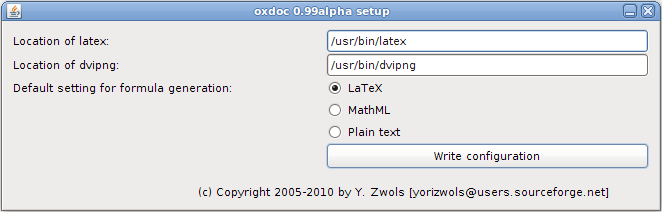
\includegraphics[scale=0.5]{setup_linux.png}
\end{center}
\item Make sure to specify the location of the {\tt latex} and {\tt dvipng} files
of your \LaTeX~installation.s
\item Click `Write configuration' to save the options to the main \oxdoc~configuration file
(i.e. a file named \oxdocxml~that is located in the `.oxdoc' subdirectory of your home directory.
\end{enumerate}

You are now ready to use \oxdoc. In the subdirectory {\tt bin}
you can find the \oxdoc~graphical user interface that helps you get started
with running \oxdoc. You may run it by typing:
\begin{quote}\tt
/opt/bin/oxdocgui
\end{quote}
You may run the command line (recommended) version of \oxdoc~by typing:
\begin{quote}\tt
/opt/bin/oxdoc
\end{quote}
It should display a short description of the program options.



